\documentclass[twoside]{article}

\usepackage{lipsum}
\usepackage[none]{hyphenat} 

\usepackage[sc]{mathpazo} 
\usepackage[T1]{fontenc} 
\linespread{1.05}
\usepackage{microtype}

\usepackage[hmarginratio=1:1,top=32mm,columnsep=20pt]{geometry}
\usepackage{multicol} 
\usepackage[hang, small,labelfont=bf,up,textfont=it,up]{caption} 
\usepackage{booktabs} 
\usepackage{float} 
\usepackage{hyperref}
\usepackage{amsmath}

\usepackage{lettrine} 
\usepackage{paralist}

\usepackage{abstract} 
\renewcommand{\abstractnamefont}{\normalfont\bfseries}
\renewcommand{\abstracttextfont}{\normalfont\small\itshape} 

\usepackage{graphicx}

\usepackage{titlesec} 
\renewcommand\thesection{\Roman{section}} 
\renewcommand\thesubsection{\Roman{subsection}} 
\titleformat{\section}[block]{\large\scshape\centering}{\thesection.}{1em}{} 
\titleformat{\subsection}[block]{\large}{\thesubsection.}{1em}{}

\usepackage{fancyhdr} 
\pagestyle{fancy} 
\fancyhead{} 
\fancyfoot{}

\fancyhead[C]{MO II $\bullet$ Tema 7 $\bullet$ C-411}
\fancyfoot[RO,LE]{\thepage}

\title{\vspace{-0.5cm}\fontsize{20pt}{10pt}\selectfont\textbf{Demanda de electricidad estoc\'astica}}

\author{
\large
\textsc{\vspace{-3cm} Alejandro Campos, Darian Dominguez, Daniel Dominguez}\\[4.5cm]
\normalsize Facultad de Matem\'atica y Computaci\'on \\
\normalsize Universidad de la Habana \\
\normalsize 2022 \\[1cm]
\vspace{-5mm}
}
\date{}


\usepackage{graphicx}
\begin{document}

\maketitle

\thispagestyle{fancy} 

\begin{center}
\textbf{Resumen}
\end{center}
\noindent \textit{Para estudiar los mercados de electricidad desregulados, se han propuesto modelos. La mayor\'ia de ellos corresponden a un llamado juego de l\'ider-seguidor en el que un Operador de Sistema Independiente (ISO) juega un papel central. Nuestro objetivo es considerar funciones de oferta cuadr\'aticas junto con las p\'erdidas de transmisi\'on en el juego multi-l\'ider-seguidor y, a partir de estas, calcular la producci\'on garantizando que su costo sea m\'inimo. Usaremos la librer\'ia de python \text{GEKKO} para lograrlo.}\\[0.5cm]

\begin{multicols}{2}



\section{Introducci\'on}

Con la desregulaci\'on y privatizaci\'on del mercado el\'ectrico en muchos pa\'ises desde mediados de la d\'ecada de 1980, han aparecido nuevos modelos en la literatura. Estos modelos se basan fundamentalmente en juegos no cooperativos que se pueden describir de la siguiente manera: el mercado de la electricidad es centralizado por un Operador de Sistema Independiente (ISO), donde cada agente ofrece su costo de producci\'on y demanda al ISO que calcula la mejor producci\'on, con el fin de minimizar el costo de esta. Esto lleva a un juego llamado multi-l\'ider-seguidor en el que cada agente se enfrenta a un problema de dos niveles. 

Los consumidores y los generadores de electricidad est\'an ubicados en diferentes nodos conectados por l\'ineas de transmisi\'on de energ\'ia. En la mayor\'ia de los modelos existentes se supone que las ofertas de los generadores siguen leyes lineales o afines. Sin embargo, es interesante considerar los mercados al contado, en los que las funciones de oferta de la generaci\'on (producci\'on) o de los consumidores (demanda) est\'an m\'as estructurados que los lineales. Por lo que, en este problema trabajamos con funciones de demanda y costo cuadr\'aticas.

Por otro lado, en algunas situaciones como transporte de larga distancia o alta intensidad, las p\'erdidas de transmisi\'on a lo largo de las l\'ineas no pueden pasarse por alto. Por ello, la influencia de las p\'erdidas de transmisi\'on en el equilibrio del sistema se ha tenido en cuenta tambi\'en en este problema. Nuestro objetivo es trabajar simult\'aneamente funciones de oferta no lineales para generadores y las p\'erdidas de transmisi\'on en la red.

En las diferentes secciones del presente trabajo nos concentraremos en explicar de una forma m\'as precisa este problema de demanda de electricidad, proponiendo un modelo matem\'atico que se ajusta a este. A este modelo le daremos soluci\'on mediante la librer\'ia \textsc{GEKKO} del lenguaje de progamaci\'on python. No sin antes explicar c\'omo esta librer\'ia resuelve los problemas de optimizaci\'on. Adem\'as, explicaremos un ejemplo muy sencillo para un mejor entendimiento de toda la teor\'ia que abordaremos. Por \'ultimo, abordaremos las distintas distribuciones para la generaci\'on de la demanda de electricidad de cada nodo.\\\\



\section{Modelo matem\'atico}

Consideramos un mercado puntual de electricidad basado en una red de transmisi\'on. Los agentes de los mercados son los productores. Cada nodo de la red est\'a compuesto por un productor y un consumidor (eventualmente con una demanda nula). Se supone que las l\'ineas de la red est\'an orientadas. Cada l\'inea tiene una capacidad de transmisi\'on m\'axima y se consideran las p\'erdidas t\'ermicas. De acuerdo a modelos cl\'asicos las p\'erdidas t\'ermicas son proporcionales al cuadrado de la transmisi\'on que fluye a lo largo de la l\'inea. 

El mercado de electricidad est\'a regulado por un operador de sistema independiente (ISO). Por lo tanto cualquier agente (como productor) proporciona al ISO una funci\'on de oferta cuadr\'atica dada por los par\'ametros $a_i$ y $b_i$. Luego, el ISO calcula el conjunto de producciones admisibles para cada nodo $i$ ($q_i$) y transmisiones entre cada nodo $i$ y $j$ ($t_{ij}$), conociendo:

\begin{itemize}
\item $N$ n\'umero de agentes del mercado de electricidad,
\item $L$ conjunto de pares $<i,j>$ que representan las l\'ineas de electricidad entre el agente $i$ y el agente $j$,
\item $L_{ij}$ coeficiente de p\'erdida t\'ermica correspondiente a la l\'inea $<i,j>$, y
\item $D_i$ demanda de electricidad correspondiente al nodo $i$
\end{itemize}

Se sabe, adem\'as, que el costo de generaci\'on de cada nodo est\'a dado por la expresi\'on $a_i q_i + b_i q_i^2$ con $i = 1, ..., N$. Donde $a_i$ y $b_i$ corresponden a la i-\'esima posici\'on de los vectores $A$ y $B$, de tama\~no $N$, conocidos. 

Por \'ultimo, el coeficiente de p\'erdida t\'ermica viene dado por $L_{ij}t_{ij}^2$ y es asumido equitativamente por los nodos $i$ y $j$.  

As\'i, el ISO, conociendo los par\'ametros anteriores, calcula $q = (q_i)_{i \in N}$ y $t = (t_{ij})_{ij \in L}$, no negativos, de forma tal que se minimice el costo total de generaci\'on y se satisfaga la demanda de electricidad de cada nodo, es decir, resolver el siguiente problema de optimizaci\'on:

{ \small
\begin{align*}
\min_{q,t} \quad \sum_{i = 1}^N a_iq_i &+ b_iq_i^2 \\
s.a. \ \ q_i &\geq 0, i = 1,...,N \\
t_{ij} &\geq 0, ij \in L \\
q_i - \sum_{k : ik \in L}{(t_{ik} + \frac{L_{ik}}{2} t_{ik}^2)} + &\sum_{k : ki \in L}{(t_{ki} - \frac{L_{ki}}{2} t_{ki}^2) \geq D_i}, \\
 &i = 1,...,N \\
\end{align*} }

En este problema la \'unica restricci\'on no trivial es la \'ultima. Esta asegura que se satisfaga la demanda de cada nodo $i$, planteando que la energ\'ia de un nodo $i$ debe ser mayor o igual que la demanda de este. En esta restricci\'on tenemos dos sumatorias, la primera representa la energ\'ia que sale de un nodo $i$, es decir, se suman los flujos de las l\'ineas de salida de este hacia otros nodos sumando, adem\'as, lo que aporta este nodo a la p\'erdida t\'ermica de dichas l\'ineas que, como se asume equitativamente, solo aporta la mitad de la p\'erdida t\'ermica. La segunda sumatoria representa la energ\'ia que entra al nodo $i$, o sea, se suman los flujos de las l\'ineas que llegan a este nodo, quitando la mitad de la p\'erdida t\'ermica que debe asumir dicho nodo en el flujo de las l\'ineas en cuesti\'on. Luego, la energ\'ia total que sale del nodo se representa con signo negativo, mientras que la que entra a este se representa con signo positivo. Por tanto, la energ\'ia de cada nodo corresponde a lo que produce menos la energ\'ia total que sale de este sumado a la energ\'ia total que llega.\\\\



\section{GEKKO}

GEKKO es un software de optimizaci\'on para ecuaciones algebraicas diferenciales y enteras mixtas. Se combina con solucionadores a gran escala para programaci\'on de enteros lineales, cuadr\'aticos, no lineales y mixtos (LP, QP, NLP, MILP, MINLP). Los modos de operaci\'on incluyen reconciliaci\'on de datos, optimizaci\'on en tiempo real, simulaci\'on din\'amica y control predictivo no lineal.

GEKKO es una abstracci\'on de alto nivel de problemas de optimizaci\'on matem\'atica. Los valores de los modelos se definen mediante constantes, par\'ametros y variables. Estos est\'an relacionados entre s\'i por intermedios o ecuaciones. Las funciones objetivas se definen para maximizar o minimizar ciertos valores. Los objetos son colecciones integradas de valores (constantes, par\'ametros y variables) y relaciones (intermedios, ecuaciones y funciones objetivas). Los objetos pueden basarse en otros objetos con relaciones orientadas a objetos.

En el back-end GEKKO compila un modelo a c\'odigo de bytes y realiza la reducci\'on del modelo en base al an\'alisis de la estructura de dispersi\'on (incidencia de variables en ecuaciones o funci\'on objetivo) del modelo. El n\'ucleo de todos los modos es el modelo no lineal. Una vez que la soluci\'on est\'a completa, se escriben los resultados en \texttt{results.json} que GEKKO vuelve a cargar en las variables de Python.

Al combinar los enfoques de los lenguajes de modelado algebraico (AML) t\'ipicos y los paquetes de control \'optimos, GEKKO facilita enormemente el desarrollo y la aplicaci\'on de herramientas como el control predicativo de modelos no lineales (NMPC), la optimizaci\'on en tiempo real (RTO) y simulaci\'on din\'amica.

Como GEKKO constituye un lenguaje de modelado algebraico (AML), nos permite plantear problemas de optimizaci\'on en modelos sencillos, basados en ecuaciones orientadas a objetos, para interactuar con potentes solucionadores de optimizaci\'on incorporados, que tienen la capacidad para ejecutar control predictivo de modelos y optimizaci\'on en tiempo real.

GEKKO, al ser un AML, facilita la interfaz entre los solucionadores avanzados y los usuarios. Los solucionadores de gama alta requieren una amplia informaci\'on sobre el problema, incluidos los l\'imites de las variables, las funciones de restricci\'on y las funciones objetivas, todo en un formato coherente. GEKKO simplifica el proceso al permitir que el modelo se escriba en un formato simple e intuitivo. El lenguaje de modelado acepta un modelo (restricciones) y un objetivo a optimizar. GEKKO maneja los enlaces al binario del solucionador, mantiene el formato requerido de los solucionadores y expone las funciones necesarias. Las llamadas de funci\'on necesarias incluyen residuales de restricci\'on, valores de funci\'on objetivo y derivadas. La mayor\'ia de los lenguajes de modelado modernos, como GEKKO, aprovechan la diferenciaci\'on autom\'atica  para facilitar gradientes exactos sin una definici\'on de derivada expl\'icita por parte del usuario.

Dado que Python est\'a dise\~nado para la legibilidad y la facilidad en lugar de la velocidad, la librer\'ia GEKKO de python se convierte en una representaci\'on de bajo nivel en el back-end de Fortran para acelerar las llamadas a funciones. La diferenciaci\'on autom\'atica proporciona los gradientes necesarios, exactos a la precisi\'on de la m\'aquina, sin trabajo adicional por parte del usuario. Luego, GEKKO interact\'ua con los solucionadores integrados de c\'odigo abierto, comerciales y personalizados a gran escala para la optimizaci\'on en el back-end. Posteriormente, los resultados de la optimizaci\'on, como ya se dijo, se vuelven a cargar en Python para facilitar el acceso y un mayor an\'alisis o manipulaci\'on.

Por tanto podemos concluir que GEKKO es una biblioteca de Python orientada a objetos que ofrece construcci\'on de modelos, herramientas de an\'alisis y optimizaci\'on que ofrece muchas ventajas. Es por ello que utilizamos GEKKO para resolver nuestro problema de optimizaci\'on del mercado de electricidad.\\\\



\section{Resoluci\'on del modelo}

Para la resoluci\'on del modelo, como afirmamos en la secci\'on anterior, nos auxiliamos de la librer\'ia GEKKO de python. La implementaci\'on se puede encontrar en \texttt{utils/solveModel.py}.

Primeramente creamos un objeto de tipo GEKKO que consistir\'a nuestro modelo y, posteriormente vamos a\~nadiendo a este las diferentes variables, restricciones y la funci\'on objetivo. Guardamos los $q_i$ en una lista de taman\~no $N$, estos son objetos de tipo \textsf{GEKKO.Var} con l\'imite inferior igual a $0$. Los $t_{ij}$ se crean de forma an\'aloga y los guardamos en una matriz de $NxN$ que contiene la variable de GEKKO si $<i,j> \in L$ y $-1$ en caso contrario. 

Desp\'ues de a\~nadir las variables a nuestro modelo, le agregamos las restricciones. En este caso, como definimos nuestras variables no negativas, solo nos queda adicionar la restricci\'on de satisfacci\'on de la demanda. Recordemos que es una restricci\'on para cada nodo, por tanto tenemos que a\~nadir $N$ restricciones. Con ayuda de \textsf{GEKKO.Equation} creamos las restricciones tal y como se definieron en la secci\'on II. Por \'ultimo, le agregamos la funci\'on objetivo al modelo como se expuso en dicha secci\'on.

Antes de resolver el modelo se define el modo de funcionamiento de GEKKO. Esta librer\'ia tiene varios modos de funcionamiento, ajustables con el par\'ametro \textsf{model.options.IMODE} que define el tipo de problema. Cada tipo de problema trata las clases de variables de manera diferente y crea ecuaciones para cumplir con el objetivo particular heredado de este. En este caso escogimos el modo 3 ya que es el estado estable para resolver problemas de optimizaci\'on en tiempo real. Finalmente, resolvemos el problema con \textsf{GEKKO.solve()}. 

La siguiente secci\'on muestra un ejemplo donde se reflejan los resultados de ejecutar la implementaci\'on antes expuesta.



\section{Ejemplo}

Veamos el siguiente ejemplo en el que tenemos $4$ agentes, que presentan las siguientes conexiones:\\

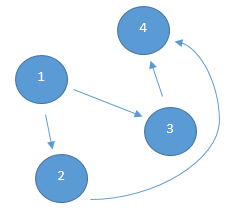
\includegraphics{img/pic_1.png} \\

Supongamos, adem\'as, que las demandas de los agentes 2 y 4 tienen demanda nula y la demanda del resto de los nodos viene dada por: $D_1 = 5$, $D_3 = 1$. Tenemos que los vectores A y B son $A = \{1, 4, 5, 8\}$, $B = \{2, 4, 4, 1\}$. Por \'ultimo, desestimemos la p\'erdida t\'ermica de todas las l\'ineas menos de la l\'inea $<1,3>$ que es igual a 2.

Ya tenemos todos los datos que necesitamos para resolver el modelo. Si le pasamos estos datos a nuestro m\'etodo \textsf{solveModel} y miramos en la consola, obtenemos:\\

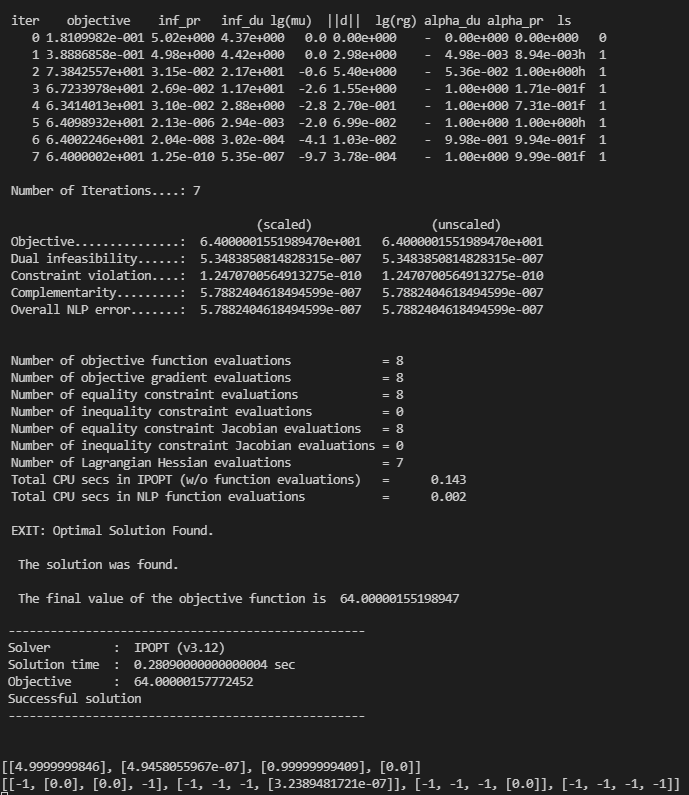
\includegraphics[scale = 0.35]{img/pic_2.png} \\

Podemos observar que llegamos a una soluci\'on optima. GEKKO nos muestra, adem\'as, algunos datos de inter\'es entre los que se encuentran la cantidad de iteraciones que se realizaron para llegar a la soluci\'on, en este caso 7. Tambi\'en notamos que muestra los detalles de cada iteraci\'on, donde podemos ver, por ejemplo, la evaluacio\'on de la funci\'on objetivo en cada una. Esta se evalu\'o 8 veces hasta obtener la soluci\'on final, al igual que su gradiente. Obteniendo un costo m\'inimo de 64 aproximadamente. El tiempo de soluci\'on fue de 0.28 segundos. 

Adem\'as de la informaci\'on que GEKKO nos brinda, imprimimos en consola los resultados de las variables. La primera lista corresponde a la producci\'on de cada nodo, mientras que la segunda corresponde con los flujos asociados a cada l\'inea. \\\\



\section{Generaci\'on de la demanda}

Seg\'un se plantea en el problema, la demanda se genera atendiendo a una distribuci\'on seleccionada por el usuario. Se deben escoger entre las siguientes distribuciones:

\begin{itemize}
\item uniforme
\item exponencial
\item gamma
\item normal
\item binaria
\item geom\'etrica
\item por escenarios
\end{itemize}

En el caso de la \'ultima se debe poner la demanda y la probabilidad con la que esta aparecer\'a. La implementaci\'on de cada una de las distribuciones anteriores se encuentra en \texttt{utils/random\_variables.py}. Todas las distribuciones que describen la demanda fueron implementadas tal cual se muestra en el cap\'itulo 5 de \cite{ross}.\\\\


\begin{thebibliography}{99}
	\bibitem{ross} Ross 2010 A First Course in Probability 8th Ed
\end{thebibliography}






\end{multicols}{2}
\end{document}